\documentclass[12pt,a4paper]{article}

\usepackage[utf8]{inputenc}
\usepackage[english]{babel}
\usepackage{a4wide}
\usepackage{index}
\usepackage{blindtext}
\usepackage[graf, intHoriz, sinLU, showDirectores]{../assets/caratula}
\usepackage{indentfirst}

\usepackage{amsmath}
\usepackage{amssymb}
\usepackage{bm}
\usepackage{hyperref}
\usepackage[dvipsnames]{xcolor} % more colors

\usepackage{pgfplots}
\usepackage{tikz}
\usetikzlibrary{arrows,backgrounds}
\usetikzlibrary{calc}
\usetikzlibrary{shapes.geometric}
\usepgflibrary{shapes.multipart}

\usepackage{adjustbox}
\usepackage{multirow}
\usepackage{array}
\usepackage{makecell}
\usepackage{subfig}
\usepackage{float}
\usepackage{tabularx,booktabs}
\usepackage{siunitx}
\usepackage{wrapfig}
\usepackage{mwe}
\usepackage{listings}
\usepackage{enumitem}

% chess typesetting
\usepackage{skak}
\usepackage{xskak}
\usepackage{wasysym} % other symbols

\usepackage{csquotes}
\usepackage[backend=biber]{biblatex}
\addbibresource{../refs.bib}

\DeclareCaptionFormat{custom}{\textbf{#1#2} #3}
\captionsetup{format=custom,labelsep=period}

\integrante{Martín Emiliano Lombardo}{}{mlombardo9@gmail.com}
\titulo{Feature set analysis for chess NNUE networks}
\fecha{\today}
\materia{Tesis de Licenciatura}
\director{Agustín Sansone}{agustinsansone7@gmail.com}
\director{Diego Fernández Slezak}{dfslezak@dc.uba.ar}

\makeindex

\begin{document}

\maketitle

\pagenumbering{gobble}
\thispagestyle{plain}
\begin{center}
\large
\textbf{Abstract}
\end{center}

\begin{center}
\parbox{15cm}{
Historically, chess engines have used highly complex functions to evaluate chess positions. Recently, efficiently updatable neural networks (NNUE) have displaced these functions without the need of human knowledge. The input of these networks are called feature sets and they take advantage of the order in which positions are evaluated in a depth-first search to save computation. \\

In this thesis, I develop a classical chess engine, where the evaluation function is replaced by a NNUE network trained with a pipeline created from scratch. The main goal of this thesis is to test novel feature sets that can improve performance. Additionally, a way of training the networks is tried using a method proposed years ago but with a higher volume and quality of data available in the post-NNUE era.
}
\end{center}

\vspace{1cm}

\begin{center}
\large
\textbf{Abstract (Spanish)}
\end{center}

\begin{center}
\parbox{15cm}{
Históricamente, los motores de ajedrez han utilizado funciones altamente complejas para evaluar posiciones de ajedrez. Recientemente, las redes neuronales eficientemente actualizables (NNUE) han desplazado a estas funciones sin necesidad de utilizar conocimiento humano. El input de estas redes se las denomina feature sets y se aprovechan del orden en que se evalúan las posiciones en una búsqueda depth-first para ahorrar cómputo. \\

En esta tesis desarrollo un motor de ajedrez clásico, en donde la función de evaluación es reemplazada por una red NNUE entrenada con un pipeline creado de cero. Esta tesis busca probar novedosos feature sets que puedan mejorar el rendimiento. Adicionalmente, se prueba una manera de entrenar las redes utilizando un método propuesto hace años pero con un volumen y calidad de datos superiores disponibles en la era post-NNUE.
}
\end{center}

\clearpage

\thispagestyle{plain}
\begin{center}
\large
\textbf{Agradecimientos}
\end{center}

:)
\clearpage


\pagenumbering{arabic}
\setcounter{page}{1}

\tableofcontents
\newpage

\section{Introduction}

% The rise of NNUEs
% https://stanford.edu/~cpiech/cs221/apps/deepBlue.html

% https://deepmind.google/discover/blog/alphazero-shedding-new-light-on-chess-shogi-and-go/
% https://crimsonpublishers.com/cojra/pdf/COJRA.000563.pdf
% https://arxiv.org/pdf/2209.11902.pdf

The development of chess engines was and continues to be a topic of study in the chess and computer communities for decades. IBM DeepBlue \cite{deepblue:2002} was the first chess machine to reach superhuman level by consistently beating the world champion, Garry Kasparov, in 1997 \cite{washingtonpost:1997}. Since then, engines have evolved in strength and complexity. \\

Chess can be modeled as a tree, where each node is a particular board configuration and the edges are legal moves for that position. With this representation, engines can use tree search algorithms to explore the tree and approximate the best move. Since the 1950s and to this date, engines have used algorithms like Minimax \cite{minimax-survey:1995} and Monte Carlo Tree Search \cite{mcts-survey:2012} (MCTS) or some of its variants \cite{tree-search-methods:2014,mcts-modifications:2022} to accomplish this.

The number of possible positions in chess is vast, estimated by Shannon \cite{shannon:1950} to be around $10^{43}$. This number is based on the average number of legal moves per position and the average game length. This makes it not feasible to explore the entire tree, so every tree search algorithm relies on having an evaluation function: a function that takes the state of the game and returns a single real number. This number is used to encompass information about the whole subtree of that position so it can be propagated up the tree, depending on the algorithm. Until a few years ago, highly complex handcrafted functions were used that were based on human knowledge about the game. \\

Until the 2010s, the development of engines advanced at a slow but consistent pace. Until 2017 that Google DeepMind published AlphaGo Zero \cite{alphagozero:2017} and its successor AlphaZero \cite{alphazero:2017,alphazero:2018} in 2018, which proved to be overwhelmingly superior (28 wins, 73 draws and 0 losses against the best engine at that time). They introduced a new approach to the development of board game engines, including chess: train a convolutional neural network with a reinforcement learning algorithm to learn to play by itself.

This change of paradigm, where the evaluation of positions is done by neural networks instead of functions built with human knowledge, altered the course of development of all modern engines (not just Go and chess). In 2018, Yu Nasu introduced the networks \reflectbox{EUNN} (or NNUE) ``Efficiently Updatable Neural-Networks'' \cite{nnue:2018} for the game Shogi. NNUE networks allow for cheap evaluations when evaluating a sequence of similar positions, making them ideal for use in depth-first search based engines. Since then, all modern engines have incorporated NNUE networks or some kind of neural network in their evaluation.

The chess engine Stockfish \cite{stockfish}, modern successor of DeepBlue with improved heuristics and running in commercial hardware is one of the strongest in the world. It incorporated NNUE networks mixed with classical evaluation in version 12\footnote[1]{\href{https://stockfishchess.org/blog/2020/introducing-nnue-evaluation/}{Introducing NNUE evaluation (Stockfish 12)}}. Since Stockfish 16.1\footnote[2]{\href{https://stockfishchess.org/blog/2024/stockfish-16-1/}{Removal of handcrafted evaluation (Stockfish 16.1)}} (2024) the evaluation is done exclusively through NNUE networks, eliminating all human aspect.

\newpage
\subsection{Thesis plan}

The main goal of this thesis is to explore different kinds of board encodings called feature sets. These encodings are the input for a NNUE network. To do so, I need a chess engine that supports neural networks with the ability to customize encodings and a way to train them.

I decided to implement a simple but capable classic engine based on well-known algorithms and optimizations, and then change the evaluation to use NNUE networks, with a versatile framework to build feature sets. Finally, I implemented a training pipeline to train the networks and measure their performance.

With the setup ready, I run multiple experiments. I propose different feature sets, train networks with them and compare their performance.

% The initial idea was to use Stockfish with the official Pytorch trainer \cite{nnue-pytorch}. However, I quickly realized that implementing some of the features sets I had in mind may be too complicated  with Stockfish's representation and the unconventional training test (PQR) that I wanted to do was impossible. This, and given that Stockfish engine and trainer codebases are huge, I felt there was too much magic involved so I turned away. I could have picked up another less complex engine written in Rust (like Marlin) and modify it, but I choose not to.
% So, I decided to implement my own engine and training pipeline from scratch.

\subsection{Source code}

The source code for this work can be found online in the following repositories:

\begin{table}[H]
\centering
\begin{tabular}{ll}
\toprule
\textbf{Repository} & \textbf{Repository} \\
\midrule
Source code & \url{https://github.com/mlomb/cs-master-thesis} \\
\LaTeX\ documents & \url{https://github.com/mlomb/cs-master-thesis-doc}
\end{tabular}
\end{table}


\section{Motor de ajedrez}

\begin{frame}
\frametitle{Motor de ajedrez}
Para evaluar las redes NNUEs es necesario un motor de ajedrez. Evaluar las redes en el vacío no se puede. \pause \\
\vspace{1em}
Buscamos construir un \textbf{motor de ajedrez clásico}, con \textbf{optimizaciones clásicas} pero \textbf{que use NNUEs} para evaluar posiciones.
\end{frame}

\begin{frame}
\frametitle{Minimax}
Tenemos una función $f$. \\ \pause
\vspace{1em}
\textbf{Primera idea}: evalúo todas las posiciones a las que me puedo mover y elijo la mejor. \\
\vspace{1em}
\pause
Pero si extendemos la idea recursivamente... es el algoritmo \textbf{minimax}.
\begin{itemize}
\item \textcolor{ForestGreen}{$\triangle$} \textbf{Maximizing nodes}: nuestro jugador.
\item \textcolor{red}{\raisebox{0.1em}{\rotatebox[origin = c]{180}{$\triangle$}}} \textbf{Minimizing nodes}: el oponente.
\end{itemize}
\end{frame}

\begin{frame}[shrink=7]
\frametitle{Minimax}
\begin{figure}
\centering
% https://tikz.dev/tikz-trees
\begin{tikzpicture}[level distance=18mm,level/.style={sibling distance=70mm/####1},line width=0.5mm,minimum size=1.5cm, inner sep=-10mm]
    % regular polygon, regular polygon sides=3
\tikzstyle{max node}=[regular polygon, regular polygon sides=3,draw=ForestGreen]
\tikzstyle{min node}=[regular polygon, regular polygon sides=3,shape border rotate=180,draw=red]
\node[max node]{-7}
child{
    node[min node]{-10} edge from parent[draw=black]
    child {
        node[max node]{10} edge from parent[draw=black]
        child {
            node[min node]{10} edge from parent[draw=black]
            child {
                node[max node]{10} edge from parent[draw=black]
            }
            child {
                node[max node]{$+\infty$} edge from parent[draw=black]
            }
        }
        child {
            node[min node]{5} edge from parent[draw=black]
            child {
                node[max node]{5} edge from parent[draw=black]
            }
        }
    }
    child {
        node[max node]{-10} edge from parent[draw=black]
        child {
            node[min node]{-10} edge from parent[draw=black]
            child {
                node[max node]{-10} edge from parent[draw=black]
            }
        }
    }
}
child {
    node[min node]{-7} edge from parent[draw=blue]
    child {
        node[max node]{5} edge from parent[draw=black]
        child {
            node[min node]{5} edge from parent[draw=black]
            child {
                node[max node]{7} edge from parent[draw=black]
            }
            child {
                node[max node]{5} edge from parent[draw=black]
            }
        }
        child {
            node[min node]{$-\infty$} edge from parent[draw=black]
            child {
                node[max node]{$-\infty$} edge from parent[draw=black]
            }
        }
    }
    child {
        node[max node]{-7} edge from parent[draw=black]
        child {
            node[min node]{-7} edge from parent[draw=black]
            child {
                node[max node]{-7} edge from parent[draw=black]
            }
            child {
                node[max node]{-5} edge from parent[draw=black]
            }
        }
    }
};
\end{tikzpicture}
\caption{Un árbol minimax de 4 de profundidad. El \enquote{mejor} movimiento para el jugador maximizador es el que lleva a la evaluación más alta, macada en \textcolor{blue}{azul}.}
\end{figure}
\end{frame}

% \begin{frame}
% \frametitle{Iterative deepening}
% No queremos hacer minimax a una profundidad fija, si no a un tiempo fijo (100 milisegundos). \\
% \vspace{1em}
% \pause
% \textbf{Iterative deepening} es una técnica que consiste en hacer minimax a profundidades crecientes, hasta que se acabe el tiempo. \\
% \vspace{1em}
% \pause
% Che pero no pierdo todo el cómputo que hice en la iteración anterior? \pause \textbf{Sí, pero...} \\
% \end{frame}

\begin{frame}
\frametitle{Optimizaciones}
\begin{itemize}
\item<1-> Poda Alpha-beta % (\href{https://mlomb.dev/slides/mcts}{anim})
\begin{itemize}
    \item cortar ramas que sabés que no se van a elegir
\end{itemize}
\item<2-> Reordenamiento de movimientos (peor caso Minimax)
\begin{itemize}
\item visitar primero los movimientos que parecen más prometedores
\end{itemize}
\item<3-> Tablas de transposición
\begin{itemize}
    \item un caché
\end{itemize}
\end{itemize}
\end{frame}

\newcommand{\white}{\fullmoon}
\newcommand{\black}{\newmoon}

\newcommand{\bigtimes}{\mathop{\raisebox{-0.5ex}{\scalebox{2}{$\times$}}}}

% https://texdoc.org/serve/chessboard/0
\newcounter{pieceindex}
\newcommand{\pieceBoard}{
    \newcount\pieceindex
    \setcounter{pieceindex}{0}
    \raisebox{-7ex}{
        \centering
        \chessboard[
            tinyboard,
            showmover=false,
            margin=false,
            padding=false,
            hlabel=false,
            vlabel=false,
            pgfstyle={text},
            %text=\fontsize{1.2ex}{1.2ex}\bfseries\sffamily \thepieceindex \stepcounter{pieceindex}, %  \currentwq
            text=\fontsize{1.2ex}{1.2ex}\bfseries\sffamily \currentwq,
            markboard
        ]
    }
}
\newcommand{\pieceRolesTable}{
    \begin{tabular}{|l|}
        \hline
        \sympawn\ Pawn \\
        \hline
        \symknight\ Knight \\
        \hline
        \symbishop\ Bishop \\
        \hline
        \symrook\ Rook \\
        \hline
        \symqueen\ Queen \\
        \hline
        \symking\ King \\
        \hline
    \end{tabular}
}
\newcommand{\pieceColorsTable}{
    \begin{tabular}{|l|}
        \hline
        $\white$ White \\
        \hline
        $\black$ Black \\
        \hline
    \end{tabular}
}

\newcommand{\featureset}[1]{\textsc{#1}}


\section{Feature sets (board encodings)}

To evaluate chess positions, the engine will use a neural network with an architecture explained in detail in the next chapter. In this chapter, I will show how to build the one-dimensional input vector for such network, which can be described entirely by a feature set.

A feature set (or feature block) is comprised of elements which represent some information about a chess position. A feature set is usually built by a cartesian product of smaller sets of features, to represent more complex patterns. Each element corresponds to a value in the input vector, which will be set to $1$ if the pattern captured by the element is present in the position (we say that the element is \textit{active}), and $0$ otherwise.

Let's consider some basic sets of features. The following sets encode positional information about the board:

\begin{center}
\begin{tabular}{cc}

$\begin{aligned}[t]
\featureset{File} &= \{a, b, ..., h\} \\
\featureset{Rank} &= \{1, 2, ..., 8\} \\
\featureset{Square} &= \{a1, a2, ..., h8\}
\end{aligned}$

&

\raisebox{-10ex}{
\chessboard[
    tinyboard,
    showmover=false,
    pgfstyle={text},
    %text=\fontsize{1.2ex}{1.2ex}\bfseries\sffamily \thepieceindex \stepcounter{pieceindex}, %  \currentwq
    text=\fontsize{1.2ex}{1.2ex}\bfseries\sffamily \currentwq,
    markboard
]
}

\end{tabular}
\end{center}

And the following encode information about the pieces:

\begin{center}
$\begin{aligned}[t]
\featureset{Role} &= \text{\{
    \sympawn\ Pawn,
    \symknight\ Knight,
    \symbishop\ Bishop,
    \symrook\ Rook,
    \symqueen\ Queen,
    \symking\ King\}}\textsuperscript{1} \\
\featureset{Color} &= \text{\{\white\ White, \black\ Black\}}
\end{aligned}$
\end{center}

\footnotetext[1]{The color of the pieces have no meaning in the definition. They are present for illustrative purposes.}

Since each set has to capture some pattern from the position, it must be stated explicitly. For example, consider the feature set $\featureset{File}_{P} \times \featureset{Color}_{P}$ where $P$ is \textit{any} piece in the board, meaning that the tuples $(file, color)$ that will be active are the ones where there is at least one piece in $file$ with the color $color$ (disregarding any other kind of information, like the piece's role). Another possible feature set could be $\featureset{File}_{P} \times \featureset{Role}_{P}$, with a similar interpretation. Note that $\featureset{Square}_Q = \featureset{File}_Q \times \featureset{Rank}_Q$ $\forall Q$. An illustration of the active features of these two feature sets for the same board is shown in Figure \ref{fig:active_features}.

\begin{figure}[H]
\centering

\begin{tabular}{cc}
\raisebox{-7ex}{
\chessboard[
    tinyboard,
    showmover=false,
    hlabel=false,
    setwhite={kc3, nc2, pa2, Pd4},
    addblack={Kc8,bh7, pa7}
]
}

&

\begin{tabular}{|c|p{4cm}|p{4cm}|p{0cm}}
\cline{2-3}
\multicolumn{1}{c|}{} & \multicolumn{2}{c|}{\centering Feature set} \\
\cline{2-3}
\multicolumn{1}{c|}{} & \centering $\featureset{File}_{P} \times \featureset{Color}_{P}$ & \centering $\featureset{File}_{P} \times \featureset{Role}_{P}$ & \\
\cline{1-3}
Active features &
(a, \white), (a, \black), (c, \black), (c, \white), (d, \white), (h, \black) &
(a, \sympawn), (c, \symking), (c, \symknight), (d, \sympawn), (h, \symbishop) \\
\cline{1-3}
\end{tabular}

\end{tabular}

\caption{Active features of the feature sets $\featureset{File}_{P} \times \featureset{Color}_{P}$ and $\featureset{File}_{P} \times \featureset{Role}_{P}$ for the same board.}
\label{fig:active_features}
\end{figure}


\subsection{Sum $\oplus$}

% what to talk about:
% we want the network to find patterns between the two sets
% some feature sets can be built merging the features of two or more sets

The sum (or concatenation) of two feature sets (often called blocks) $\featureset{A}$ and $\featureset{B}$, denoted by $\featureset{A} \oplus \featureset{B}$, is a new feature set comprised of the elements of both sets $\featureset{A}$ and $\featureset{B}$. These elements do not interfere with each other, even if they share basic elements (e.g. h, 8, \symrook, \black), they \textbf{must} have different interpretations.
For example, given the feature sets $\featureset{File}_{W}$ where $W$ is any white piece in the board and $\featureset{File}_{B}$ where $B$ is any black piece in the board, the feature set $\featureset{File}_{W} \oplus \featureset{File}_{B}$ will have the basic elements $\{a, b, ..., h\}$ for both white and black pieces, but each with a different interpretation. Note that the notation presented in this work is not standard.

The sum operator is useful when we want to let the network find patterns combining information between two sets of features.

\subsection{Indexing}

The input to the network is a one-dimensional vector, so we need a way to map the tuples (elements are trivial) in a feature set to elements in the input vector. The correct index for a tuple is computed using the order of the sets in the cartesian product and the size of each set, like strides in a multi-dimensional array. For this to work, each element in a set $S$ must correspond to a number between $0$ and $|S| - 1$. For example, the feature set $A \times B \times C$ has $|A| \times |B| \times |C|$ elements, and the tuple $(a, b, c)$ is mapped to the element indexed at $a \times |B| \times |C| + b \times |C| + c$. The same striding logic applies to feature sets built with the sum operator, recursively.

\subsection{Feature sets}

In this section, I will define two of the most important feature sets known and used extensively in existing engines.

\subsubsection{\mdseries\featureset{All}}

This feature set is the most natural encoding for a chess position. It is called \enquote{All} because it captures all the pieces. There is a one-to-one mapping between pieces in the board and features:

\begin{center}
    $\featureset{All} = \featureset{Square}_{P} \times \featureset{Role}_{P} \times \featureset{Color}_{P}$ \\
    for every $P$ piece in the board \\
\end{center}

Tuples in this set are \textit{active} if there is a piece in the board that matches the role, color and position of the tuple. For example, the tuple $(e4, \sympawn, \white)$ is active if there is a white pawn in the square e4. This way, for every possible piece, in every possible position, there is a feature. The set has $64*6*2=$\textbf{ 768 features}, which makes it very small and it is very easy to compute which features are active.

\subsubsection{\mdseries\featureset{King-All}}

Another feature set built on top of $\featureset{All}$ is the \featureset{King-All} feature set, or \enquote{KA} for short. For each possible position of the king of the side to move, it captures all the pieces in the board ($\featureset{All}$):

\begin{center}
    $\featureset{King-All} = \featureset{Square}_{K} \times \featureset{All}_{P}$ \\
    where $K$ is the king of the side to move and\\
    $P$ is every piece in the board \\
\end{center}

This encoding allows the network to understand better the position of the pieces in relation to the king, which is very tied to the evaluation of the position.

The number of features is $64*768=$ \textbf{49152 features}. There is a variation of this feature set called \enquote{KP} which is the same but it does not consider the enemy king, reducing the amount of features to 40960. There are other variations, such as \featureset{KAv2} or notably \featureset{KAv2\_hm} that is currently the latest feature set used by Stockfish 16.1.

The features in this set are easy to compute like in $\featureset{All}$, but since the number of features is much larger, it is a lot harder to train and use in practice. I will restrain this work to smaller feature sets that are easier to manage.

\subsection{Dead features}

Consider the $\featureset{All}$ feature set. For every position, role and color each piece could be, there is a feature. There are 16 tuples in the set that will never be active: (a8..h8, \sympawn, \white) and (a1..h1, \sympawn, \black) that correspond to the white pawns in the last rank and the black pawns in the first rank. This is because pawns promote to another piece when they reach the opponent side of the board, so no pawns will ever be found there. Effectively, these will be dead neurons in the network, but this way we can keep the indexing straightforward. Most feature sets will have dead features, and the same logic applies.

\section{Efficiently updatable neural networks}

NNUE (\reflectbox{NNUE} Efficiently updatable neural network) is a neural network architecture that allows for very fast subsequent evaluations for minimal input changes. It was invented for Shogi by Yu Nasu in 2018 \cite{nnue:2018}, later adapted to Chess for use in Stockfish in 2019 and may be used in other board games as well. Most of the information described in this chapter can be found in the excellent Stockfish NNUE documentation \cite{nnue-pytorch}. \\

NNUE operates in the following principles:

\begin{itemize}
    \item \textbf{Input sparsity}: The network should have a relatively low amount of non-zero inputs, determined by the chosen feature set. The presented feature sets have between 0.1\% and 2\% of non-zero inputs for a typical position. Having a low amount of non-zero inputs places a low upper bound on the time required to evaluate the network in its entirety, which can happen using some feature sets like \featureset{HalfKP} that triggers a complete refresh when the king is moved.
    \item \textbf{Efficient updates}: From one evaluation to the next, the number of inputs changes should be minimal. This allows for the most expensive part of the network to be efficiently updated, instead of recomputed from scratch.
    \item \textbf{Simple architecture}: The network should be composed of a few and simple operators, that can be efficiently implemented with low-precision arithmetic in integer domain using CPU hardware. [no accelerators, aggresive quantization techniques]
\end{itemize}

[tradeoff between speed and accuracy]

\subsection{Layers}

For this thesis, I have chosen to use the standard NNUE architecture, which consist of multiple linear (fully connected) layers and clipped ReLU activations. In the literature, there are other architectures that make use of polling layers, sigmoid activations and others, but since this work is about experimenting with feature sets and training methods, I have chosen to stick with the standard architecture.

\paragraph[short]{Linear layer} A linear layer is a matrix multiplication followed by a bias addition. It takes \textbf{in\_features} input values and produces \textbf{out\_features} output values. The operation is $\bm{y} = \bm{W} \bm{x} + \bm{b}$, where:

\begin{enumerate}
\item $\bm{x}$ the input column vector of shape \textbf{in\_features}.
\item $\bm{W}$ the weight matrix of shape (\textbf{out\_features}, \textbf{in\_features}).
\item $\bm{b}$ the bias column vector of shape \textbf{out\_features}.
\item $\bm{y}$ the output column vector of shape \textbf{out\_features}.
\end{enumerate}

The operation $\bm{W} \bm{x}$ can be simplified to \enquote{if $\bm{x_i}$ is not zero, take the column $\bm{A_i}$, multiply it by $\bm{x_i}$ and add it to the result}. This means that we can skip the processing of columns that have a zero input, as depicted in Figure \ref{fig:linear_comparison}.

\begin{figure}[H]
\centering
\subfloat[\centering Linear layer]{{\includegraphics[width=5cm]{../assets/nnue/mv.pdf} }}%
\qquad
\subfloat[\centering Linear layer with sparse inputs]{{\includegraphics[width=5cm]{../assets/nnue/mvs.pdf} }}%
\caption{Linear layer operation comparison. Figures from \cite{nnue-pytorch}.}
\label{fig:linear_comparison}
\end{figure}

In the case of the first layer, the input is a very sparse one-hot encoded vector. This means that very few columns will have to be processed and the multiplication can be skipped altogether, due all inputs being either 0 or 1.

\paragraph[short]{Clipped ReLU} This is a simple activation that clips the output in the range $[0, 1]$. The operation is $\bm{y=\min(\max(x,0),1)}$.
The output of this activation function is the input for the next layer, and because of the aggresive quantization that will be described later, it is necessary to restrain the values so it does not overflow. \\

\subsection{Efficient updates}

When running a depth-first search algorithm, the state of the position is updated every time the algorithm \textit{makes} and \textit{unmakes} moves, usually before and after the recursion.
NNUEs are designed to work with this kind of search, since every time the algorithm \textit{makes} (or \textit{unmakes}) a move, the changes in the position are minimal (at most two pieces are affected), meaning that the amount of features becoming active or inactive is minimal as well. This is depicted in Figure \ref{fig:updates_tree}.

\begin{figure}[H]
\centering
\storechessboardstyle{3x3}{tinyboard,maxfield=c3,margin=false,showmover=false,hlabel=true,vlabel=true,pgfstyle=color,color=blue}
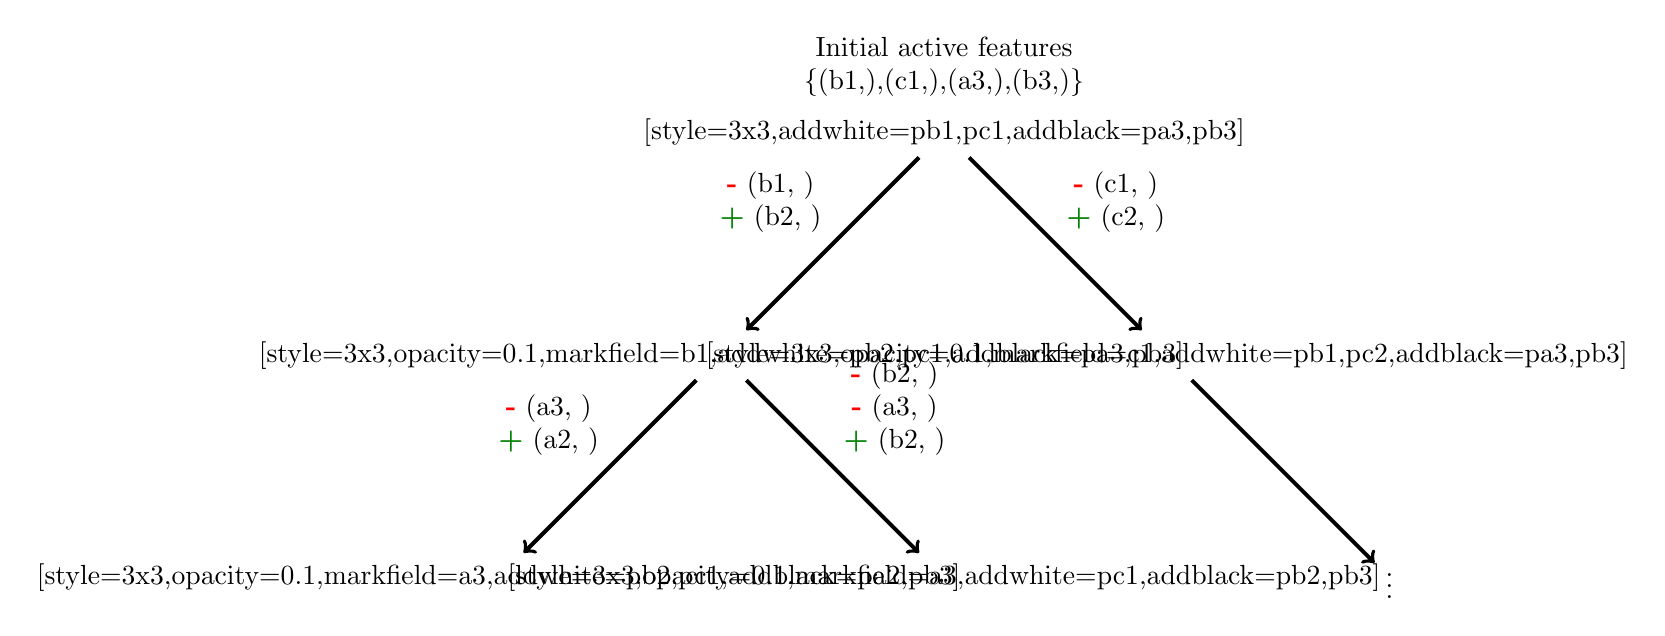
\begin{tikzpicture}[
    node distance=4cm,
    line width=0.5mm,
    auto
]

    \node[label={[align=center]Initial active features \\ \{(b1,\white),(c1,\white),(a3,\black),(b3,\black)\}}] (A) {\chessboard[style=3x3,addwhite={pb1,pc1},addblack={pa3,pb3}]};

    % childs of A
    \node (B) [below left of=A] {\chessboard[style=3x3,opacity=0.1,markfield={b1},addwhite={pb2,pc1},addblack={pa3,pb3}]};
    \node (C) [below right of=A] {\chessboard[style=3x3,opacity=0.1,markfield={c1},addwhite={pb1,pc2},addblack={pa3,pb3}]};

    % childs of B
    \node (D) [below left of=B] {\chessboard[style=3x3,opacity=0.1,markfield={a3},addwhite={pb2,pc1},addblack={pa2,pb3}]};
    \node (E) [below right of=B] {\chessboard[style=3x3,opacity=0.1,markfield={a3},addwhite={pc1},addblack={pb2,pb3}]};

    % childs of C
    \node (F) [below right of=C] {\vdots};

    % arrows of A
    \path[<-] (B) edge node[align=center] {\textbf{{\color{Red}-}} (b1, \white) \\ \textbf{{\color{Green}+}} (b2, \white)} (A);
    \path[->] (A) edge node[align=center] {\textbf{{\color{Red}-}} (c1, \white) \\ \textbf{{\color{Green}+}} (c2, \white)} (C);
    
    % arrows of B
    \path[<-] (D) edge node[align=center] {\textbf{{\color{Red}-}} (a3, \black) \\ \textbf{{\color{Green}+}} (a2, \black)} (B);
    \path[->] (B) edge node[align=center] {\textbf{{\color{Red}-}} (b2, \white) \\ \textbf{{\color{Red}-}} (a3, \black) \\ \textbf{{\color{Green}+}} (b2, \black)} (E);

    % arrows of C
    \path[<-] (F) edge node[align=center] {} (C);

\end{tikzpicture}
\caption{Partial tree of feature updates (\textcolor{Red}{removals} and \textcolor{Green}{additions}) for $\featureset{SQUARE}_P \times \featureset{COLOR}_P$ (white's point of view) in a simplified 3x3 pawn-only board.}
\label{fig:updates_tree}
\end{figure}

To take advantage of this during search, instead of computing all the features active in a position and then evaluate the network in its entirety, we can \textbf{accumulate} the output of the first linear layer and update it with when the position changes. Linear layers can be computed adding the corresponding columns of the weight matrix into the output, so when a feature becomes active or inactive, we can add or subtract the corresponding column to the output. When the evaluation is needed, only the following layers (usually small) have to be computed. \\

Recall that the way I defined feature sets, they always encode the position from white's point of view. This means that its not possible to use the same \textbf{accumulator} for both players. So when running the search, we have to keep two accumulators, one for white and one for black, where the black board is flipped and has the colors swapped to match the point of view.
[mencionar que tambien realmente es porque queremos codificar el que mueve y se va swapeando]

[agregar grafico de black → white board → encode, para mostrar como se flipea / swapea. arriba el white → encode; poner los features activos quizas?]

\subsection{Network}

The network will be composed of four linear layers $L_1$ through $L_4$, each but the last one followed by a clipped ReLU activation $C_1$ through $C_3$. The network has two inputs: it takes the encoding (feature set) of a position from each player's point of view. Each encoding is passed through the same $L_1$ layer (same weights) and then the output is concatenated before passing it through the rest of the network. [hablar de que no es la unica alternativa?] The first layer can be seen as a feature transformer, and it must share weights to allow for efficient updates. The network can be described as follows: \\

$\bm{N}$: number of features in the feature set

\begin{enumerate}
\itemsep-0.2em
\item $L_1 \times 2$: Linear from $\bm{N}$ to $\bm{M}$ ($\bm{W_1}$ weight, $\bm{b_1}$ bias)
\item $C_1$: Clipped ReLU of $\bm{2 * M}$
\itemsep0.2em
\item $L_2$: Linear from $\bm{2 * M}$ to $\bm{O}$ ($\bm{W_2}$ weight, $\bm{b_2}$ bias)
\itemsep-0.2em
\item $C_2$: Clipped ReLU of $\bm{O}$
\itemsep0.2em
\item $L_3$: Linear from $\bm{O}$ to $\bm{P}$ ($\bm{W_3}$ weight, $\bm{b_3}$ bias)
\itemsep-0.2em
\item $C_3$: Clipped ReLU of $\bm{P}$
\itemsep0.2em
\item $L_4$: Linear from $\bm{P}$ to $\bm{1}$ ($\bm{W_4}$ weight, $\bm{b_4}$ bias)
\end{enumerate}


The size of each layer is not fixed since it is a hyperparameter I will experiment with. The network architecture is depicted in Figure \ref{fig:network}, with example parameters.

\begin{figure}[H]
\centering
\makebox[\textwidth]{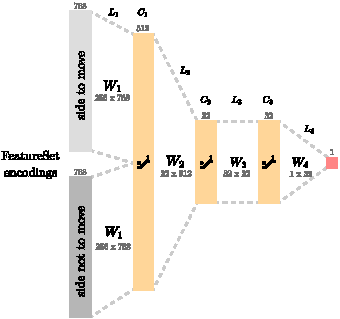
\includegraphics[width=12cm]{../assets/nnue/network.pdf}}
\caption{Neural network architecture with $\bm{N}=768$, $\bm{M}=256$, $\bm{O}=\bm{P}=32$. Not to scale.}
\label{fig:network}
\end{figure}

During search, the first layer $L_1$ is replaced by two accumualtors to take advantage of efficient updates, as explained in the previous section. Figure \ref{fig:incr_update} depicts how the output of both accumulators is concatenated depending on which player is moving, to later be passed through the rest of the network which are computed as usual. 

\begin{figure}[H]
\centering
\makebox[\textwidth]{\includegraphics[width=\textwidth]{../assets/nnue/incremental_update.pdf}}
\caption{Concatenation of the first layer's output after a move is made.}
\label{fig:incr_update}
\end{figure}

\subsection{Quantization}

% https://github.com/official-stockfish/nnue-pytorch/blob/master/docs/nnue.md#quantization

Quantization is the process of converting the operations and parameters of a network to a lower precision. It is a step performed after all training has been done, which do happen in float domain. Floating point operations are too slow to achieve maximum performance, as it sacrifices too much speed. Quantizing the network to integer domain will inevitable introduce some error, but it far outweights the performance gain. In general, the deeper the network, the more error is accumulated, but since NNUEs are very shallow by design, the error is negligible.

The objective is to take advantage of modern CPUs that allow doing low-precision integer arithmetic in parallel with 8, 16, 32 or even 64 8-bit integer values at a time. To achieve this, the best is to use the smallest integer type possible everywhere, to process more values at once.

\subsubsection{Stockfish quantization scheme}

\def\int#1{\texttt{int#1}}

In this thesis, I will use the same quantization scheme used in the engine Stockfish \cite{nnue-pytorch}. It uses \int{8} $[-128, 127]$ for inputs and weights, and \int{16} $[-32768, 32767]$ where \int{8} is not possible.
To convert the float values to integer, we need to multiply the weights and biases by some constant to translate them to a different range of values. Each layer is different, so I'll go through each one.

%\begin{figure}[H]
%\centering
%\makebox[\textwidth]{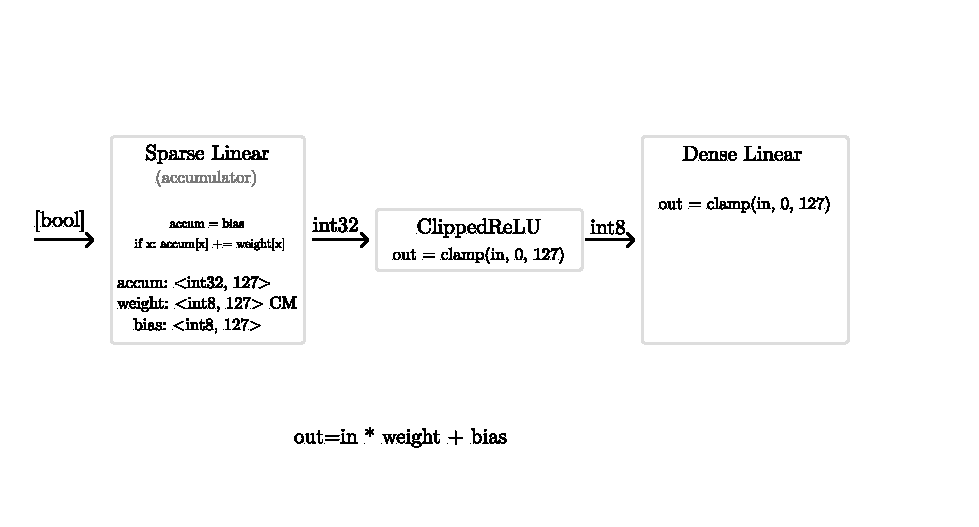
\includegraphics[width=\textwidth]{../%assets/nnue/quantization.pdf}}
%\caption{Simplified network showcasing all layers with %quantization values}
%\label{fig:quantization}
%\end{figure}

\paragraph[short]{ClippedReLU} The output of the activation in float domain is in the range $[0, 1]$ and we want to use \int{8} in the quantized version, so we can clamp in the range [0, 127] instead. The input data type may change depending on the previous layer: if it comes from the accumulator, it will be \int{32}, and if it comes from a linear layer, it will be \int{16}.

ACTIVATION RANGE SCALING = 127

% \paragraph[short]{Input} Since we are using accumualtors, there is not a real input to the model.
% Inputs are quantized to 8 bits, so the range of values is $-128..127$. Since the inputs are hot encoded, the float values are 0.0 or 1.0, so the quantized values are either 0 or 127.

\paragraph[short]{Accumulator} The purpose of this layer is to accumulate rows of the first layer's weight matrix. Later linear layers expect the input in \int{8}, 


. Since the output of this layer will be the input for the next linear layer and it has the ClippedReLU activation, the output will also be in 8 bits.
But since we are accumulating 8 bits values and


and to output a clipped value of 8 bits for the next layer.

we can't accumulate using 8 bits since it would overflow.

COLUMN MAJOR

\paragraph[short]{Linear layer}
The input to this layer will be scaled to the activation range because it takes the output of the previous ClippedReLU activation. We want the output to also be scaled to the activation rango so it can be passed to the next. The activation range scaling is $s_a=127$, as explained before.

To convert the weights to \int{8}, we must scale them by some factor $s_W=64$ (value used in Stockfish). The value $s_W$ depends on how much precision we want to keep, but if it is too large the weights will be limited in magnitude. The range of the weights in floating point is then determined by $\pm \frac{s_a}{s_W}=\frac{127}{64}=1.984375$, and to make sure weights don't overflow, it is necessary to clip them to this range during training. The value $s_W$ also determinates the minimum representable weight step, which is $\frac{1}{s_W}=\frac{1}{64}=0.015625$.

The linear layer operation with the scaling factors applied looks like:

\begin{equation}
\begin{aligned}
s_a s_W \bm{y} &= (s_W \bm{W}) (s_a \bm{x}) + s_a s_W \bm{b} \\
\end{aligned}
\end{equation}
\begin{equation}
\begin{aligned}
s_a \bm{y} &= \frac{(s_W \bm{W}) (s_a \bm{x}) + s_a s_W \bm{b}}{s_W} \\
\end{aligned}
\end{equation}

From that equation we can extract that, to obtain the result we want, which is the output of the layer scaled to the activation range ($s_a \bm{y}$), we must divide the result of the operation by $s_W$ (2). Also that the bias must be scaled by $(s_a s_W)$. \\

The last linear layer is a bit different since there is no activation afterwards, so we don't want the output to be scaled to the activation range $(s_a)$. To be consistent with the Stockfish engine, the output values should be in the range $[-10000,10000]$.



% The scaling factor for the output of the last layer is $s_o=9600$.

$s_o=9600$

\begin{equation}
\begin{aligned}
s_o ((s_a \bm{x}) (s_W \bm{w}) + s_a s_W \bm{b}) = s_a s_W s_o \bm{y}
\end{aligned}
\end{equation}







no se tiene el mismo problema que en el accumulator layer porque la multiplicacion en SIMD se hace en 32 bits (osea sin hacer overflow), para despues aplicar clippedrelu a eso.

. \\

asd

\subsection{Implementation}

The Stockfish repository provides an AVX2 implementation of the mathematical operations in C++. They have been carefully ported to Rust for this thesis. The implementation was tested using the Pytorch model as reference (output match).


\begin{figure}[H]
\centering
\includegraphics[width=12cm]{./dynamic/output/quant_errors.pdf}
\caption{Absolute error of the quantized model compared to the float model. N=50000}
\label{fig:quant_errors}
\end{figure}

Error

\section{Training}

Given a feature set, the network architecture is completely defined, along with how to encode a position into its inputs. This section will describes two proposed methods to train the networks, each with its own loss function and training dataset.

\subsection{Source dataset}

Data is needed to train the network. The proposal for the thesis was to use the Lichess database \cite{lichessdb}, which provides a CC0 database with all the games ever played on the site, then score the positions using Stockfish. After some initial experiments, the networks were not performing as expected. Upon further reaserch I found out that I was working with datasets too small for this task (order of hundreds of millions). I needed a larger dataset (order of \textbf{dozens of billions}), but it was impractical for me to generate it. Fortunately, I can use the same dataset that Stockfish uses to train its networks \cite{sf_nnue_dataset}, which should work well. Specifically, I went with the dataset used to train the first stage of the main network for Stockfish 16.1, which is 135GB of compressed \texttt{binpack} files. It was built by running Stockfish at 5000 nodes per move on multiple opening books. Later stages use datasets generated by Leela Chess Zero (LC0), which is more expensive to compute but has a higher quality evaluations.

The \texttt{binpack} format is a very efficient format to store samples yet very complex to decode. Fortunately, Stockfish provides a tool to export this data into a text format. I had to modify it to export it in the format I wanted. I changed the \texttt{emitPlainEntry} function in \texttt{nnue\_data\_binpack\_format.h} to the code in Appendix \ref{appendix:emitPlainEntry}. The resulting file was 2.59TB in size and contained \textbf{48.4 billion samples}. There is one sample per line with the format:

\begin{center}
\begin{tabular}{|cp{0.0005cm}cp{0.0005cm}c|}
\hline
\textbf{FEN\footnotemark} & , & \textbf{Score} & , & \textbf{Best move} \\
\hline
\end{tabular}
\end{center}

\footnotetext{Standard notation to describe positions of a chess game. It is a sequence of ASCII characters.}

The file was too big to be practical and it would wear off my SSD, so I made a tool to compact the data into a similar format. The new format expoits the fact that samples in a row belong to the same game. This means that contiguous FENs are a move from a previous one, so it stores the move instead of the FEN:

\begin{center}
\begin{tabular}{|cp{0.0005cm}cp{0.0005cm}c|}
\hline
\textbf{FEN} & , & \textbf{Score} & , & \textbf{Best move} \\
\hline
\end{tabular}
(
\begin{tabular}{|p{0.0005cm}cp{0.0005cm}cp{0.0005cm}c|}
\hline
, & \textbf{Actual move} & , & \textbf{Score} & , & \textbf{Best move} \\
\hline
\end{tabular}
) *\footnote{Repeated zero or more times.}
\end{center}

As you can see, the new format is compatible with the last one, so only one reader was implemented. After compacting the data, the file went down to a manageable 522GB. Also, reading a single FEN and later apply moves to it is much faster than parsing a FEN every time. \\

There are many positions in the dataset that are known to not be good for training. Remember that the engine is doing quiescent search, so it does a smaller search looking for quiet positions to evaluate. This means that positions where the best move is a capture, or there is a check are filtered out when building the training batch. \\

Each training method will generate a new derived dataset based on this samples.

% Lichess is a free online site to play chess, and thankfully it provides a CC0 database \cite{lichessdb} with all the games ever played on the site. It consists of serveral compressed PGN files\footnote{Portable Game Notation: a textual format to store chess games (moves and metadata)} splitted by month since 2013, that add up to $1.71$TB compressed. The whole database contains over 5.5 billion games, that equates to around 200 billion positions. In practice, that many positions are too much to handle so I'll use only a fraction of them and take only one sample per game to increase the diversity of positions.

% The Lichess database also provides a database of puzzles
% hablar de esto en otro lado (results? eval?)

% A single game can have lots of positions, most of which are shared with millions of other games, mostly during the early game. This is a problem of its own: trying to sample positions from a game with a suitable distribution. In this work, I have chosen to only consider positions 20 half-moves into the game.

\subsection{Method 1: Score target}

The main method to train the network will use the scores provided in the dataset as target. I expect the networks to learn to predict the evaluation of a position as Stockfish would do.

\setcounter{secnumdepth}{4}
\subsubsection{Score-space to WDL-space}

Scores are values ranging from -10000 to 10000. [hablar de que score vs performance ajusta a una sigmoid]
[hablar de que se necesita una escala]

% I guess it is to steer the old network to the new one while making 
% The evaluations from Stockfish are in centipawns, which is not the exact number the network has to use as target.
% decir que no usamos el outcome de la partida para el score

\subsubsection{Loss function}

The loss function is a mean square errror with a power of 2.6 (the value used by the Stockfish's official trainer) given by

% q = (output / out_scaling).sigmoid()
% p = (target / in_scaling).sigmoid()
% loss = torch.pow(torch.abs(p - q), 2.6).mean()

\[
L(y,f(x,\bm{W}))= \left| \sigma\left(\frac{y}{\text{scale}_{\text{in}}}\right) - \sigma\left(\frac{f(x,\bm{W})}{\text{scale}_{\text{out}}}\right) \right| ^{2.6}
\]


where\dots

\begin{enumerate}
\itemsep0em
\item $y$ is the target score.
\item $f$ is the model.
\item $\bm{W}$ are the parameters of the model.
\item $x$ is the input (encoded feature set).
\item $\sigma$ is the sigmoid function.
\item $\text{scale}_{\text{in}}$, $\text{scale}_{\text{out}}$ are the scaling factors of the scores.
\end{enumerate}

\subsection{Method 2: PQR triplets}

This is an additional technique I wanted to try, described in \cite{dlchess:2014}. The method is based in the assumption that moves in the dataset are optimal. In the blog they used human moves from the Lichess database \cite{lichessdb}, so they rely in that humans make optimal or near-optimal moves most of the time, even if they are amateurs. In my case I will use Stockfish moves, which are extremely good. This method does not use the scores provided, it will have to learn them from scratch. Of course this is way harder to train but I'm curious to see how far the following idea can go.

Remember that we are trying to obtain a function $f$ (the model) to give an evaluation of a position. The idea is based on the following two principles:

\begin{enumerate}
\item For two position in succession $p \rightarrow q$ observed in the game, we will have $f(p)=-f(q)$. This comes from the fact that the game is zero-sum.
\item Going from $p$, not to $q$, but to a \textit{random} position $p \rightarrow r$, we must have $f(r) > f(q)$ because the random move is better for the next player and worse for the player that made the move.
\end{enumerate}

If this reasonable assumptions hold, a loss function that expresses the equality and inequality can be built.

% Consider an optimal $f$, that outputs $-1,0,1$ depending on who wins.
% With infinite compute, $f$ would be the result of running minimax to the end of the game, since minimax always finds optimal moves.

\subsubsection{Loss function}

The loss function is the log likelihood of the inequalities: $f(r) > f(q)$, $f(p) > - f(q)$ and $f(p) < -f(q)$. The last two are a way to express the equality $f(p)=-f(q)$. The loss function is given by

% p = output[:,0] / out_scaling
% q = output[:,1] / out_scaling
% r = output[:,2] / out_scaling
% a = -torch.log(torch.sigmoid(q - r)).mean()
% b = -torch.log(torch.sigmoid((p + q))).mean()
% c = -torch.log(torch.sigmoid((-q - p))).mean()
% loss = a + b + c

\begin{align*}
L(x_p, x_q, x_r, \bm{W})=
& -\log\left(\sigma(q - r)\right) \\
& -\log\left(\sigma(p + q)\right) \\
& -\log\left(\sigma(-(p + q))\right)
\end{align*}

where\dots

\begin{enumerate}
\itemsep0em
\item $
p = \frac{f(x_p, \bm{W})}{\text{scale}_{\text{out}}},\text{ }
q = \frac{f(x_q, \bm{W})}{\text{scale}_{\text{out}}},\text{ }
r = \frac{f(x_r, \bm{W})}{\text{scale}_{\text{out}}}
$
\item $f$ is the model.
\item $\bm{W}$ are the parameters of the model.
\item $x_i$ is the input (encoded feature set) for the $i \in \{p,q,r\}$ position.
\item $\sigma$ is the sigmoid function.
\item $\text{scale}_{\text{out}}$ are the scaling factors of the scores.
\end{enumerate}

It is important to note that quantization is happening in this method too, so the output of the model must be scaled appropriately.

[siento que falta explicar algo en esta seccion]

\subsection{Setup}

[a esta seccion se le pueden agregar mil cosas]

% [multithreaded, perf]
% decir que en "All" tengo 450 it/s (7.3M pos/sec)


The project is written in two languages: Rust and Python. The Rust part is used to process dataset files, generate statistics and provide final training batches for Python to consume. The Python part defines the Pytorch model, runs the training loop, quantizes the model and runs the evaluations.


The training process is started by running a Python script (\texttt{scrips/train.py}) and it requires to define the model architecture (number of neurons on each layer), general training parameters (learning rate, batch size, epochs, checkpoints, etc) and the feature set to use, which in turn determines the size of the batches. For example, if PQR is used, the size of a sample is 3 times the size of the feature set times two (because it is siamese), and if it is eval (short for score \textbf{eval}uations), it is the size of the feature set times two plus 1 for the target score.

To orchestrate training runs, the platform Weights and Biases (WandB) is used. It provides automatic sweeping of hyperparameter, logging of metrics and visualizations. Results are exported from the platform in CSV and then processed by Python scripts. \\

% multithreading
AAAA M \\

The training data has to be converted to an actual tensor of floats to be consumed by Pytorch. This is done by a Rust subprocess running the subcommand \texttt{samples-service} that read the training data files and generates training batches for the specified feature set in a shared memory buffer. The Python script copies the data from the buffer at the start of each iteration, allowing Rust to generate the next batch (in the CPU) while Pytorch is training the current batch (in the GPU). To coordinate the memory access between the two processes, a single byte is sent using standard I/O.

Given that the input vector is multiple-hot encoded, the data written by the Rust process are not float values. Instead, they are 64-bit integers acting as a bitset. Before passing the vector to the model, it is expanded into floats. This means 64 floats can be packed into a single 64-bit integer, meaning a \textbf{96.875\%} reduction in memory usage (from 256 to 8 bytes). The speedup obtained by this optimization was substantial. The compression can be further improved using sparse tensors, but it is not implemented in this work. \\

[evaluation?]

\newcommand{\depiction}[1]{\parbox{0.7cm}{\includegraphics[height=0.7cm]{../assets/depictions/#1.pdf}}}
\newcommand{\depictionSM}[1]{\parbox{0.6cm}{\includegraphics[height=0.6cm]{../assets/depictions/#1.pdf}}}


\section{Experiments and results}

Now that the engine, the tools and the methodology are defined, we can proceed to the experiments. Experiments will be divided in three sections: motivation, experiment and results. The motivation will explain why I think the experiment is relevant and present possible hypothesis. The experiment will describe configurations to train different models, how they will be evaluated and what are my expectations. The results will present the data, explain whether my hypothesis was correct or not and give a brief conclusion. \\

Every model's training configuration is defined by the following variables:

\begin{itemize}
\item \textbf{Feature set}: Determinates the encoding of the position, and thus the number of inputs of the model. It conditions which patterns the network can learn. Experimenting with this is the main focus of this thesis.

\item \textbf{Network architecture}: The size of each layer in the network. The first layer (L1) is the feature transformer and it is efficiently updated. The following layer (L2) should be tiny due the NNUE architecture. The size of the model (its complexity) roughly determinates how many patterns the network can learn.

\item \textbf{Dataset}: The positions to train on. The dataset used is explained in detail in chapter 5. In summary, there are 48.5 billion positions to train on and the dataset remains constant across all runs. About 5 million positions are used for validation.

% no me gusta la palabra computed...
\item \textbf{Training method}: Can choose to use either score targets or PQR triplets. This determinates the format of the samples as well as the loss function. All experiments will train using score targets, unless specified. Methods were explained in detail in chapter 5.

\item \textbf{Training hyperparameters}: The usual machine learning hyperparameters for training, such as batch size, learning rate and scheduler. I used the same epoch size used in Stockfish, where each epoch is 100 million positions. Each training run will last for 256 epochs, which means the network is trained in 25.6 billion positions (recall that some of the original 48.5 billion dataset are skipped).
\end{itemize}

Once training is completed, the models will be evaluated depending on the experiment. To assess the performance of a model or to compare a set of models, the following indicators are used:

\begin{itemize}
\item \textbf{Loss}: The training and validation loss are used to detect overfitting and other possible problems. It can't be used to measure the performance of a model. Bigger models must have much better predictions to outweight the cost of having slower inferences and thus less node visits. It's a tradeoff.

\item \textbf{Puzzle accuracy}: The percentage of moves correctly predicted by the engine in Lichess puzzles. Each puzzle may contain multiple moves, and the engine has 100ms per move. Since the engine is not that strong, it does not solve 100\% of puzzles like many other engines do, so I expect differences in this metric to be good indicators. A small set of puzzles is used during training as (a very bad) proxy for the engine's strength, to have early insight of the strength and to detect catastrophic failures that did arise. A bigger set of 85000 puzzles is used after training.

\item \textbf{Relative ELO rating}: A tournament is played between different models to determine their relative strength. Ordo is used to compute the ELO of each model based on the results of the tournament. This is the most important metric, as it is the most reliable way to compare the strength of engines.

% \item \textbf{Inference performance (infs/s)}:

\item \textbf{Training duration}: The amount of time it takes to train a model. This is a one time operation and it does not affect the performance of a model. However, it does condition which and how many experiments I can run.
\end{itemize}

All networks that are not in the first experiment (the baseline), are trained 4 times and a tournament is played between the epoch 192 and 256 of each network (8 networks in total). I have observed a difference of 30 elo points between runs, so this step is crucial to have sensible results. In the appendix are the results of each run and tournament.


\begin{frame}
\frametitle{Setup de training}
Recapitulando... ¿Qué hay que definir para entrenar una red? \pause
\begin{itemize}
\item (variable) \textbf{Feature set}: determina el encoding \pause
\item \checkmark\ \textbf{Dataset}: datos de entrenamiento \pause
\item \checkmark\ \textbf{Método de entrenamiento}: PQR/target scores; determina el formato de las muestras y la loss function  \pause
\item ? \textbf{Arquitectura de la red}: el tamaño de cada capa; $L_1$ y $L_2$ \pause
\item ? \textbf{Hiperparámetros}: learning rate, batch size, epochs, etc.
\end{itemize}
\end{frame}

\begin{frame}
\frametitle{Setup de evaluación}
¿Cómo evalúo el performance de una red entrenada? \pause
\begin{itemize}
\item \textbf{Loss} (train y val.): indica la calidad de las predicciones.
\begin{itemize}
    \item Permite detectar overfitting y otros problemas \pause
\end{itemize}
\item \textbf{Puzzle accuracy}: porcentaje de movimientos acertados en puzzles de Lichess.
\begin{itemize}
    \item Sólo hay un movimiento correcto
    \item Proxy (muy malo) de la fuerza de la red \pause
\end{itemize}
\item \textbf{Elo relativo}: la medida más común para comparar engines.
\begin{itemize}
    \item Se realizan torneos de 100ms por movimiento
    \item El elo es calculado a partir de Ordo
\end{itemize}
\end{itemize}
\end{frame}

\begin{frame}
\frametitle{Baseline: motivación}
Busco fijar el setup de entrenamiento con valores razonables \pause
Queda por determinar\dots
\begin{itemize}
\item La arquitectura de la red: $L_1$ y $L_2$
\item Los hiperparámetros
\end{itemize}
\end{frame}

\begin{frame}
\frametitle{Baseline: hiperparámetros}
Los hiperparámetros fueron seleccionados en base al trainer oficial de Stockfish:
\begin{itemize}
\item \textbf{Learning rate}: 0.0005
\item \textbf{Exponential decay}: 0.99
\item \textbf{Batch size}: 16384
\item \textbf{Epoch size}: 100 million
\begin{itemize}
    \item cada epoch realiza 6104 batches
\end{itemize}
\item \textbf{Epochs}: 256
\begin{itemize}
    \item cada run observa \textit{25.6 billion} samples
\end{itemize}
\end{itemize}
\end{frame}


\begin{frame}
\frametitle{Baseline: experimento}
Sólo queda buscar parámetros $L1$ y $L2$ razonables. Realizo una búsqueda en grilla con:
\begin{itemize}
\item $L1$ $\in \{256, 512, 1024, 2048\}$
\item $L2$ $\in \{32, 64, 128, 256\}$
\end{itemize}
El feature set a utilizar es \featureset{All}[768].
\end{frame}

\begin{frame}
\frametitle{Baseline: resultados}
\begin{figure}
\centering
\makebox[\textwidth]{\includegraphics[width=0.93\textwidth]{../thesis/dynamic/output/baseline_heatmaps.pdf}}
\end{figure}
\end{frame}

\begin{frame}
\frametitle{Baseline: conclusión}
\begin{itemize}
\item \textbf{L2=32}. El performance cae dramáticamente si L2 aumenta, utilizo el más bajo.
\begin{itemize}
    \item Sería buena idea probar valores más chicos de L2. \pause
\end{itemize}
\item \textbf{L1=512}. Es el mejor valor para L2=64 y L2=128, y en margen de error para L2=32.
\begin{itemize}
    \item Además es el más rápido de entrenar.
\end{itemize}
\end{itemize}
\end{frame}


\begin{frame}
\frametitle{Axis encoding: motivación}

\begin{figure}[h]
\centering
\subfloat[\centering $\white$ White]{{\includegraphics[width=4.4cm]{../assets/results/piece_weights/white_rook_weights.png} }}%
\qquad
\subfloat[\centering $\black$ Black]{{\includegraphics[width=4.4cm]{../assets/results/piece_weights/black_rook_weights.png} }}%
\caption{Weights of \textbf{a neuron} in the L1 layer, which are connected to features in \featureset{All} where the role is $\rook$ Rook. The intensity represents the weight value, and the color represents the sign (although not relevant).}
\label{fig:rook_weights}
\end{figure}

\end{frame}


\begin{frame}
\frametitle{Pairwise axes: motivación}

\storechessboardstyle{smallvert}{
    tinyboard,
    maxfield=a8,
    showmover=false,
    hmargin=false,
    hlabel=false,
    boardfontsize=15pt,
}

\newcommand{\raiseby}{-11.5ex}

\begin{figure}
\centering

\begin{tabular}{ccc}

\raisebox{\raiseby}{\chessboard[
    style=smallvert,
    clearboard,
    addblack={Ra7},
    addwhite={na3,pa4},
]}
\raisebox{\raiseby}{\chessboard[
    style=smallvert,
    clearboard,
    addblack={Ra8},
    addwhite={na2,pa3},
]}
\raisebox{\raiseby}{\chessboard[
    style=smallvert,
    clearboard,
    addblack={Ra6},
    addwhite={na3,pa4},
]}
\raisebox{\raiseby}{\chessboard[
    style=smallvert,
    clearboard,
    addblack={Ra5},
    addwhite={na1,pa3},
]}
\raisebox{\raiseby}{\chessboard[
    style=smallvert,
    clearboard,
    addblack={Ra6},
    addwhite={na2,pa3},
]}

$\hdots$

&
$ \rightarrow$
&

\raisebox{-9.5ex}{\chessboard[
    blackfieldcolor=white,
    blackfieldmaskcolor=white,
    maxfield=a8,
    style=smallvert,
    vlabel=false,
    border=false,
    trim=false,
    opacity=0.6,
    clearboard,
    addblack={Ra6},
    addwhite={na2,pa4},
    %
    color=red,
    shortenend=1.88ex,shortenstart=1.88ex, % espacio
    padding=-1ex,
    markstyle=leftborder,
    linewidth=0.4ex,
    markregion=a4-a6,
    linewidth=1.6ex,
    pgfstyle=circle,
    markfields={a4,a6},
    %
    color=blue,
    shortenend=1.88ex,shortenstart=1.88ex, % espacio
    padding=-1ex,
    markstyle=leftborder,
    linewidth=0.4ex,
    markregion=a2-a4,
    linewidth=1.6ex,
    pgfstyle=circle,
    markfields={a2,a4},
    %
]}

\\

\makecell{Configuraciones distintas,\\situaciones similares} &  & \makecell{Las mismas dos features\\(par rojo y par azul)}

\end{tabular}
\end{figure}
\end{frame}

\begin{frame}
\frametitle{Pairwise axes: motivación}
Comparando con el experimento anterior, es más específico en vez de más general:
\begin{center}
\enquote{\textit{there is a $\white$ White $\rook$ Rook in the 4th rank}} \\
vs. \\
\enquote{\textit{there is a $\black$ Black $\rook$ Rook next to a $\white$ White $\sympawn$ Pawn in the \enquote{a} file}}
\end{center}
\end{frame}

\begin{frame}
\frametitle{Pairwise axes: experimento}
\begin{table}
\small
\centering
\begin{adjustbox}{max width=\textwidth}
\begin{tabular}{ccccc}
\toprule
\bf D. & \bf \makecell{Block\\name} & \bf Definition & \bf \makecell{Num. of\\features} \\
\toprule
\depiction{PH} & PH & \makecell{
\vspace{0.2cm}
$(\featureset{Ranks} \times (\featureset{Roles} \times \featureset{Colors}) \times (\featureset{Roles} \times \featureset{Colors}))_{P}$ \\
P($\langle r, r_1, c_1, r_2, c_2 \rangle$): there is a piece in rank $r$ with role $r_1$\\ and color $c_1$ to the left of a piece with role $r_2$ and color $c_2$
} & 1152 \\
\toprule
\depiction{PV} & PV & \makecell{
\vspace{0.2cm}
$(\featureset{Files} \times (\featureset{Roles} \times \featureset{Colors}) \times (\featureset{Roles} \times \featureset{Colors}))_Q$ \\
Q($\langle f, r_1, c_1, r_2, c_2 \rangle$): there is a piece in file $f$ with role $r_1$\\ and color $c_1$ below a piece with role $r_2$ and color $c_2$
} & 1152 \\
\bottomrule
\end{tabular}
\end{adjustbox}
\end{table}
\end{frame}

\begin{frame}
\frametitle{Pairwise axes: experimento}
\begin{figure}[h]
\centering
\begin{adjustbox}{max width=\textwidth}
\begin{tabular}{cc}

\raisebox{-7ex}{\chessboard[
    setfen=2r4k/p5p1/Kpqp3p/8/1PP2Q2/P2P1RP1/8/8 b - - 12 45,
    showmover=false,
    opacity=0.6,
    %
    % TEMPLATE HORIZONTAL
    %color=red,
    %shortenend=1.88ex,shortenstart=1.88ex, % espacio
    %padding=-1ex,
    %markstyle=topborder,
    %linewidth=0.4ex,
    %markregion=d6-d3,
    %linewidth=1.6ex,
    %pgfstyle=circle,
    %markfields={d6,d3},
    %
    color=red,
    shortenend=1.88ex,shortenstart=1.88ex, % espacio
    padding=-1ex,
    markstyle=topborder,
    linewidth=0.4ex,
    markregion=a3-d3,
    linewidth=1.6ex,
    pgfstyle=circle,
    markfields={a3,d3},
    %
    color=red,
    shortenend=1.88ex,shortenstart=1.88ex, % espacio
    padding=-1ex,
    markstyle=topborder,
    linewidth=0.4ex,
    markregion=f3-g3,
    linewidth=1.6ex,
    pgfstyle=circle,
    markfields={f3,g3},
    %
    color=blue,
    shortenend=1.88ex,shortenstart=1.88ex, % espacio
    padding=-1ex,
    markstyle=topborder,
    linewidth=0.4ex,
    markregion=d3-f3,
    linewidth=1.6ex,
    pgfstyle=circle,
    markfields={d3,f3},
    %
    color=red,
    shortenend=1.88ex,shortenstart=1.88ex, % espacio
    padding=-1ex,
    markstyle=topborder,
    linewidth=0.4ex,
    markregion=b4-c4,
    linewidth=1.6ex,
    pgfstyle=circle,
    markfields={b4,c4},
    %
    color=blue,
    shortenend=1.88ex,shortenstart=1.88ex, % espacio
    padding=-1ex,
    markstyle=topborder,
    linewidth=0.4ex,
    markregion=c4-f4,
    linewidth=1.6ex,
    pgfstyle=circle,
    markfields={c4,f4},
    %
    color=red,
    shortenend=1.88ex,shortenstart=1.88ex, % espacio
    padding=-1ex,
    markstyle=topborder,
    linewidth=0.4ex,
    markregion=a6-b6,
    linewidth=1.6ex,
    pgfstyle=circle,
    markfields={a6,b6},
    %
    color=red,
    shortenend=1.88ex,shortenstart=1.88ex, % espacio
    padding=-1ex,
    markstyle=topborder,
    linewidth=0.4ex,
    markregion=c6-d6,
    linewidth=1.6ex,
    pgfstyle=circle,
    markfields={c6,d6},
    %
    color=blue,
    shortenend=1.88ex,shortenstart=1.88ex, % espacio
    padding=-1ex,
    markstyle=topborder,
    linewidth=0.4ex,
    markregion=b6-c6,
    linewidth=1.6ex,
    pgfstyle=circle,
    markfields={b6,c6},
    %
    color=blue,
    shortenend=1.88ex,shortenstart=1.88ex, % espacio
    padding=-1ex,
    markstyle=topborder,
    linewidth=0.4ex,
    markregion=d6-h6,
    linewidth=1.6ex,
    pgfstyle=circle,
    markfields={d6,h6},
    %
    color=red,
    shortenend=1.88ex,shortenstart=1.88ex, % espacio
    padding=-1ex,
    markstyle=topborder,
    linewidth=0.4ex,
    markregion=a7-g7,
    linewidth=1.6ex,
    pgfstyle=circle,
    markfields={a7,g7},
    %
    color=blue,
    shortenend=1.88ex,shortenstart=1.88ex, % espacio
    padding=-1ex,
    markstyle=topborder,
    linewidth=0.4ex,
    markregion=c8-h8,
    linewidth=1.6ex,
    pgfstyle=circle,
    markfields={c8,h8},
]}

&

\raisebox{-7ex}{\chessboard[
    setfen=2r4k/p5p1/Kpqp3p/8/1PP2Q2/P2P1RP1/8/8 b - - 12 45,
    showmover=false,
    opacity=0.6,
    %
    % TEMPLATE VERTICAL
    %color=red,
    %shortenend=1.88ex,shortenstart=1.88ex, % espacio
    %padding=-1ex,
    %markstyle=leftborder,
    %linewidth=0.4ex,
    %markregion=d6-d3,
    %linewidth=1.6ex,
    %pgfstyle=circle,
    %markfields={d6,d3},
    %
    color=red,
    shortenend=1.88ex,shortenstart=1.88ex, % espacio
    padding=-1ex,
    markstyle=leftborder,
    linewidth=0.4ex,
    markregion=a3-a6,
    linewidth=1.6ex,
    pgfstyle=circle,
    markfields={a3,a6},
    %
    color=blue,
    shortenend=1.88ex,shortenstart=1.88ex, % espacio
    padding=-1ex,
    markstyle=leftborder,
    linewidth=0.4ex,
    markregion=a6-a7,
    linewidth=1.6ex,
    pgfstyle=circle,
    markfields={a6,a7},
    %
    color=red,
    shortenend=1.88ex,shortenstart=1.88ex, % espacio
    padding=-1ex,
    markstyle=leftborder,
    linewidth=0.4ex,
    markregion=b4-b6,
    linewidth=1.6ex,
    pgfstyle=circle,
    markfields={b4,b6},
    %
    color=red,
    shortenend=1.88ex,shortenstart=1.88ex, % espacio
    padding=-1ex,
    markstyle=leftborder,
    linewidth=0.4ex,
    markregion=c4-c6,
    linewidth=1.6ex,
    pgfstyle=circle,
    markfields={c4,c6},
    %
    color=blue,
    shortenend=1.88ex,shortenstart=1.88ex, % espacio
    padding=-1ex,
    markstyle=leftborder,
    linewidth=0.4ex,
    markregion=c6-c8,
    linewidth=1.6ex,
    pgfstyle=circle,
    markfields={c6,c8},
    %
    color=red,
    shortenend=1.88ex,shortenstart=1.88ex, % espacio
    padding=-1ex,
    markstyle=leftborder,
    linewidth=0.4ex,
    markregion=d3-d6,
    linewidth=1.6ex,
    pgfstyle=circle,
    markfields={d3,d6},
    %
    color=red,
    shortenend=1.88ex,shortenstart=1.88ex, % espacio
    padding=-1ex,
    markstyle=leftborder,
    linewidth=0.4ex,
    markregion=f3-f4,
    linewidth=1.6ex,
    pgfstyle=circle,
    markfields={f3,f4},
    %
    color=red,
    shortenend=1.88ex,shortenstart=1.88ex, % espacio
    padding=-1ex,
    markstyle=leftborder,
    linewidth=0.4ex,
    markregion=g3-g7,
    linewidth=1.6ex,
    pgfstyle=circle,
    markfields={g3,g7},
    %
    color=red,
    shortenend=1.88ex,shortenstart=1.88ex, % espacio
    padding=-1ex,
    markstyle=leftborder,
    linewidth=0.4ex,
    markregion=h6-h8,
    linewidth=1.6ex,
    pgfstyle=circle,
    markfields={h6,h8},
]}


\\

\makecell{\depiction{PH} Pairwise horizontal (\featureset{PH})} &
\makecell{\depiction{PV} Pairwise vertical (\featureset{PV})}

\end{tabular}
\end{adjustbox}
\end{figure}
\end{frame}


\begin{frame}
\frametitle{Pairwise axes: experimento}
Los feature sets a entrenar son:
\begin{itemize}
\item \featureset{All} $\oplus$ \featureset{PH} (1920 features)
\item \featureset{All} $\oplus$ \featureset{PV} (1920 features)
\item \featureset{All} $\oplus$ \featureset{PH} $\oplus$ \featureset{PV} (3072 features)
\end{itemize}
\end{frame}

\begin{frame}
\frametitle{Pairwise axes: resultados}
\begin{table}
\centering
\begin{tabular}{ccccc}
\toprule
\bf Feature set  & \bf \makecell{Number\\of features} & \makecell{\bf Val. loss\\\textit{min}} & \makecell{\bf Rating\\\textit{elo (rel. to \featureset{All})}} \\
\toprule
\featureset{All} (reference) & 768 & 0.003134 & \textbf{0.0} \\
\midrule
\featureset{All} $\oplus$ \depiction{PH} & 1920 & 0.003033 & -38.2 $\pm$ 4.8 \\
\midrule
\featureset{All} $\oplus$ \depiction{PV} & 1920 & 0.002946 & -8.4 $\pm$ 5.0 \\
\midrule
\featureset{All} $\oplus$ \depiction{PH} $\oplus$ \depiction{PV} & 3072 & \textbf{0.002868} & -37.6 $\pm$ 4.9 \\
\bottomrule
\end{tabular}
\end{table}
\begin{itemize}
    \item Reducir el número de pairs puede llevar a una mejora por sobre \featureset{All} (ej. $\sympawn$)
\end{itemize}
\end{frame}


\noindent\rule{\textwidth}{1pt}

\vspace{0.2cm}
Up to this point, I have been trying to encode the position of the pieces in different or smarter ways, with no avail. It may seem that the network is able to extract all the information it needs from the most basic \featureset{All} feature set. Making the information available in another form makes no difference, as opposed to what I originally thought.

Further experiments will focus on features not related to the position of the pieces, but to other aspects of the game, inspired by hand crafted evaluations.

\noindent\rule{\textwidth}{1pt}


\subsection{Mobility}

\textbf{Motivation.} Mobility in chess is a measure of the available moves a player can make in a given position. The idea is that if a player has more available moves, the position is stronger. In \cite{slater:1950} it was shown that there is a strong correlation between a player's mobility and the number of games won. This metric has been used extensively in hand crafted evaluations, and I propose to include this information as features for the neural network. \\

\textbf{Experiment.} There are two ways to go about encoding mobility:

\begin{itemize}
\item \textbf{Bitsets (per piece type):} Provide the exact squares each piece type can move to. The number of features would be $64 * 6 * 2 = 768$. The problem with this approach is not the amount of features, but the number of updates to the accumulator per move is very high, which slows down the search.

\begin{figure}[H]
\centering

\begin{tabular}{ccccc}

\raisebox{-7ex}{\chessboard[
    setfen=r5k1/1b1p1ppp/p7/1p1Q4/2p1r3/PP4Pq/BBP2b1P/R4R1K w - - 0 20,
    tinyboard,
    showmover=false,
]}
&

\raisebox{-7ex}{\chessboard[
    tinyboard,
    showmover=false,
    setwhite={ba2,bb2},
    pgfstyle=color,
    opacity=0.8,
    color=blue,
    markfield={b1,c1,c3,d4,e5,f6,g7}
]}

&

\raisebox{-7ex}{\chessboard[
    tinyboard,
    showmover=false,
    addblack={Bb7,Bf2},
    pgfstyle=color,
    opacity=0.8,
    color=blue,
    markfield={c8,c6,d5,a7,b6,c5,d4,e3,e1,g1,g3}
]}

&

\raisebox{-7ex}{\chessboard[
    tinyboard,
    showmover=false,
    setwhite={qd5},
    pgfstyle=color,
    opacity=0.8,
    color=blue,
    markfield={d6,d7,e6,f7,e5,f5,g5,h5,e4,d4,d3,d2,d1,c4,c5,b5,c6,b7}
]}

& $\hdots$

\\

Board &
\makecell{\white White\\\symbishop\ Bishop} &
\makecell{\black Black\\\symbishop\ Bishop} &
\makecell{\white White\\\symqueen\ Queen}

\end{tabular}
\end{figure}


\item \textbf{Counts (per piece type):} Use the number of available moves per piece type as features. This means having a feature for each possible count value, which are a lot less feature updates. To find which values to include as features I computed the total mobility for each piece role in 2 billion boards, shown in figure \ref{fig:mobility}. From the data we can extract the range of values to use as features:

\begin{table}[H]
\centering
\begin{tabular}{c|c|c}
\toprule
\textbf{Piece role} & \textbf{Min} & \textbf{Max} \\
\midrule
\sympawn\ Pawn & 0 & 8+ \\
\symknight\ Knight & 0 & 15+ \\
\symbishop\ Bishop & 0 & 16+ \\
\symrook\ Rook & 0 & 25+ \\
\symqueen\ Queen & 0 & 25+ \\
\symking\ King & 0 & 8 \\
\bottomrule
\end{tabular}
\end{table}

\begin{figure}[H]
\centering
\makebox[\textwidth]{\includegraphics[width=\textwidth]{./dynamic/output/mobility.pdf}}
\caption{Total mobility values for each piece on the board. Computed using 2 billion boards. The value 0 for the \symknight\ Knight, \symbishop\ Bishop, \symrook\ Rook and \symqueen\ Queen has been excluded from the plot, as it is very common.}
\label{fig:mobility}
\end{figure}
\end{itemize}

Each approach was implemented as a block:

\begin{table}[H]
\caption{Mobility feature blocks}
\label{tab:mobility_blocks}
\centering

\begin{tabular}{ccc}
\toprule
\bf Block name & \bf Definition & \bf Number of features \\
\toprule
MB & \makecell{
\vspace{0.2cm}
($\featureset{Squares} \times \featureset{Roles} \times \featureset{Colors})_P$ \\
P($\langle s, r, c \rangle$): there is a piece of role $r$\\ and color $c$ that \textbf{can move to} square $s$
} & 768 \\
\toprule
MC & \makecell{
\vspace{0.2cm}
$(\{0, 1, \hdots\} \times \featureset{Roles} \times \featureset{Colors})_{P}$\\
P($\langle m, r, c \rangle$): the value of mobility for\\
a piece of role $r$ and color $c$ is $m$
} & 206 \\
\bottomrule
\end{tabular}
\end{table}

The blocks will be combined with the \featureset{All} feature set. Neither of the blocks can be used alone, since they do not carry the information to deduce every piece on the board (trivially).

The feature sets to be trained and evaluated are \featureset{All} $\oplus$ \featureset{MB} (1536 features) and \featureset{All} $\oplus$ \featureset{MC} (974 features). Like prior experiments, a network will be trained for each feature set and evaluated in a tournament. \\

\textbf{Results.} The results in table \ref{tab:mobility_results} show that the blocks did not provide features of enough quality to improve the network predictions enough to overcome the cost of making more feature updates. I have underestimated the cost of a feature update, that was not a problem in previous experiments. The block \featureset{MB} has, in average, 10.03 feature updates per move and the block \featureset{MC} has 3.82 (see Appendix \ref{appendix:fs}). In comparison, the \featureset{All} feature set has 1.58 feature updates per move. Even though the block \featureset{MB} has almost 3 times the number of feature updates, it has a better performance than \featureset{MC}. This is attributed to having a 7\% lower loss, which compensates the cost of the updates. \\

\begin{table}[H]
\caption{Mobility encodings results}
\label{tab:mobility_results}
\centering

\begin{tabular}{ccccc}
\toprule
\bf Feature set  & \bf \makecell{Number\\of features} & \makecell{\bf Val. loss\\\textit{min}} & \makecell{\bf Rating\\\textit{elo (rel. to \featureset{All})}} \\
\toprule
\featureset{All} (reference) & 768 & 0.003134 & \textbf{0.0} \\
\midrule
\featureset{All} $\oplus$ \featureset{MB} & 1536 & 0.002824 & -260.9 $\pm$ 5.4 \\
\midrule
\featureset{All} $\oplus$ \featureset{MC} & 974 & 0.003032 & -280.9 $\pm$ 5.6 \\
\bottomrule
\end{tabular}
\end{table}


\begin{frame}
\frametitle{PQR}
:)
\end{frame}


%\subsection{Active neurons}
%medir si hay feature sets que no usen neuronas, que esto disparo el uso de HalfTopK
%average number of features enabled by feature set (cantidad y porcentaje)
%measure updates per move average and refreshes average per FS
%[ESTO PONERLO EN EL APPENDIX]


%%%%%%%%%%%%%%%%%%%%%%%%%%%%%%%%%%%%%%%%%%%
%%%%%%%%%%%%%%%%%%%%%%%%%%%%%%%%%%%%%%%%%%%
%%%%%%%%%%%%%%%%%%%%%%%%%%%%%%%%%%%%%%%%%%%
%%%%%%%%%%%%%%%%%%%%%%%%%%%%%%%%%%%%%%%%%%%
%%%%%%%%%%%%%%%%%%%%%%%%%%%%%%%%%%%%%%%%%%%
%%%%%%%%%%%%%%%%%%%%%%%%%%%%%%%%%%%%%%%%%%%
%%%%%%%%%%%%%%%%%%%%%%%%%%%%%%%%%%%%%%%%%%%
%%%%%%%%%%%%%%%%%%%%%%%%%%%%%%%%%%%%%%%%%%%
%%%%%%%%%%%%%%%%%%%%%%%%%%%%%%%%%%%%%%%%%%%
%%%%%%%%%%%%%%%%%%%%%%%%%%%%%%%%%%%%%%%%%%%
%%%%%%%%%%%%%%%%%%%%%%%%%%%%%%%%%%%%%%%%%%%


% \noindent\makebox[\linewidth]{\rule{\paperwidth}{0.4pt}}
% 
% Esto de abajo son notas. No se si hacerlo o no... quizas es mucho
% 
% \noindent\makebox[\linewidth]{\rule{\paperwidth}{0.4pt}}
% 
% \subsection{Attacks / Threats}
% 
% as bitsets per piece type
% number of attacks
% 
% \subsection{mas supongo?}
% 
% \subsection{Symmetry? / Relativity?}
% 
% \textbf{Motivation.}
% 
% BUCKETING
% 
% Medir el impacto de agregar simetría al fs. Red mas chica, inf mas rapida, mejor perf?
% 
% probar simetria, eventualmente probar con el mejor feature set de arriba, a ver si mejora poniendo a cada bloque individual simetria
% 
% \featureset{Half-Relative(H|V|HV)King-Piece}?
% 
% inspired by KP, build features relative to the position of the $\king$ King
% 
% \subsection{Statistical features?}
% 
% Define \featureset{k-All-All}
% 
% \featureset{King-All} is a subset of \featureset{All-All}.
% 
% Top P
% 
% Hacer un subset de \featureset{AA} (589824).
% 
% \begin{itemize}
% \item Destilar?
% \item Probar si es lo mismo quedarse con el TOP K de las mas comunes o con las que dice el performance.
% \item Catboost? PCA?
% \end{itemize}

\section{Final words}
\subsection{Conclusions}
\subsection{Future work}


% prunning feature sets? quizas no ayuda, solo para training, no se. ver bien

% lo ideal de un feature set son patrones que NO se den en simultáneo? asi podes aprender mas usando menos neuronas

future work: hacer que no sea uniforme el sampling de las posiciones para armar los datasets

future work: triplet loss?

deduplication de posiciones (al computar el score de Stockfish)


\newpage
\printbibliography

\appendix

\section{Appendix}

Runtime may be affected by other processes running on the machine, since it was my personal computer. They are listed here for reference only.

\subsection{Baseline runs}
\label{appendix:baseline}

\begin{tabular}{@{} cccccccc @{}} \toprule
\multirow{2}{*}{\bf Feature set} & \multicolumn{3}{c}{\bf Train hyperparams} & \multicolumn{2}{c@{}}{\bf Network} & \multirow{2}{*}{\makecell{\bf Val loss\\\textit{min}}} & \multirow{2}{*}{\makecell{\bf Runtime\\\textit{hh:mm:ss}}} \\
\cmidrule(lr){2-4} \cmidrule(l){5-6}
& \bf Batch & \bf LR & \bf Gamma & \bf L1 & \bf L2 & \\
\midrule
    \featureset{HV} & 16384 & 5e-04 & 0.99 & 256 & 32 & 0.00351 & 1:53:59 \\
\featureset{HV} & 16384 & 5e-04 & 0.99 & 256 & 64 & 0.00342 & 1:54:56 \\
\featureset{HV} & 16384 & 5e-04 & 0.99 & 256 & 128 & 0.00330 & 1:52:29 \\
\featureset{HV} & 16384 & 5e-04 & 0.99 & 256 & 256 & 0.00319 & 2:29:26 \\
\featureset{HV} & 16384 & 5e-04 & 0.99 & 512 & 32 & 0.00309 & 1:54:28 \\
\featureset{HV} & 16384 & 5e-04 & 0.99 & 512 & 64 & 0.00300 & 1:53:44 \\
\featureset{HV} & 16384 & 5e-04 & 0.99 & 512 & 128 & 0.00290 & 1:51:06 \\
\featureset{HV} & 16384 & 5e-04 & 0.99 & 512 & 256 & 0.00279 & 1:51:17 \\
\featureset{HV} & 16384 & 5e-04 & 0.99 & 1024 & 32 & 0.00268 & 2:15:18 \\
\featureset{HV} & 16384 & 5e-04 & 0.99 & 1024 & 64 & 0.00265 & 2:03:41 \\
\featureset{HV} & 16384 & 5e-04 & 0.99 & 1024 & 128 & 0.00257 & 2:06:39 \\
\featureset{HV} & 16384 & 5e-04 & 0.99 & 1024 & 256 & 0.00246 & 2:32:47 \\
\featureset{HV} & 16384 & 5e-04 & 0.99 & 2048 & 32 & 0.00241 & 3:11:56 \\
\featureset{HV} & 16384 & 5e-04 & 0.99 & 2048 & 64 & 0.00238 & 3:12:46 \\
\featureset{HV} & 16384 & 5e-04 & 0.99 & 2048 & 128 & 0.00234 & 3:29:07 \\
\featureset{HV} & 16384 & 5e-04 & 0.99 & 2048 & 256 & \textbf{0.00221} & 3:27:47 \\
\bottomrule \end{tabular}




\end{document}


% https://ctan.dcc.uchile.cl/info/symbols/comprehensive/symbols-a4.pdf
